\begin{prob}
    Suppose the graph shown below is a directed, weighted graph in which all of the
    edge weights are positive.

    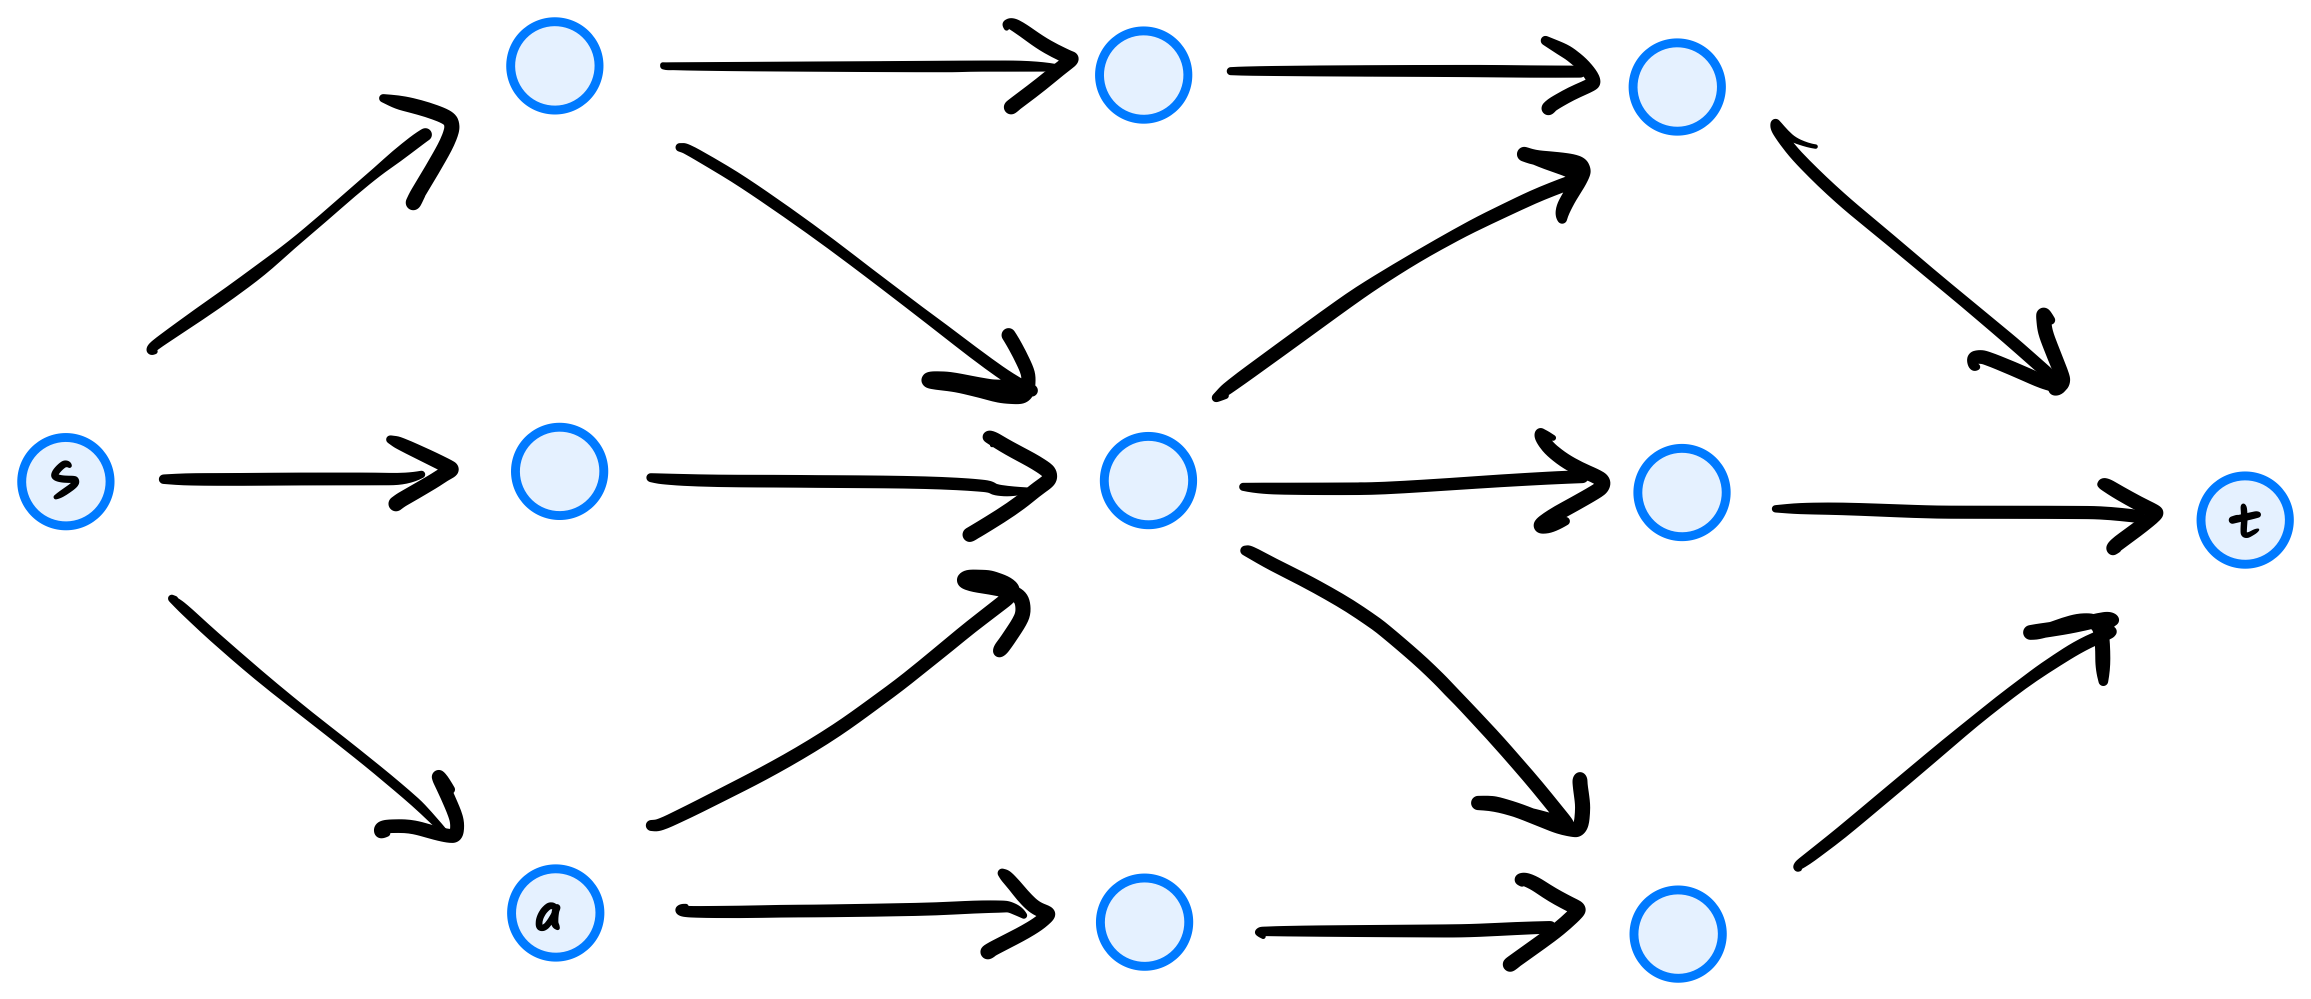
\includegraphics[width=.9\textwidth]{./fig/g7.png}

    Suppose Dijkstra's algorithm is run on this graph. True or False: it is possible
    for the edge weights to be such that node $t$ is popped from the priority queue
    before node $a$.

    \Tf{}

\end{prob}
